\documentclass{article}

\usepackage{geometry}
\usepackage{amsmath}
\usepackage{graphicx}
\usepackage{listings}
\usepackage{hyperref}
\usepackage{multicol}
\usepackage{fancyhdr}
\pagestyle{fancy}
\hypersetup{ colorlinks=true, linkcolor=black, filecolor=magenta, urlcolor=cyan}
\geometry{ a4paper, total={170mm,257mm}, top=20mm, right=20mm, bottom=20mm, left=20mm}
\setlength{\parindent}{0pt}
\setlength{\parskip}{1em}
\renewcommand{\headrulewidth}{0pt}
\lhead{Competitive Programming - Arkavidia VI}
\fancyfoot[CE,CO]{\thepage}
\lstset{
    basicstyle=\ttfamily\small,
    columns=fixed,
    extendedchars=true,
    breaklines=true,
    tabsize=2,
    prebreak=\raisebox{0ex}[0ex][0ex]{\ensuremath{\hookleftarrow}},
    frame=none,
    showtabs=false,
    showspaces=false,
    showstringspaces=false,
    prebreak={},
    keywordstyle=\color[rgb]{0.627,0.126,0.941},
    commentstyle=\color[rgb]{0.133,0.545,0.133},
    stringstyle=\color[rgb]{01,0,0},
    captionpos=t,
    escapeinside={(\%}{\%)}
}

\begin{document}

\begin{center}
    \section*{Sebuah Pola Bilangan} % ganti judul soal

    \begin{tabular}{ | c c | }
        \hline
        Batas Waktu  & 1s \\    % jangan lupa ganti time limit
        Batas Memori & 64MB \\  % jangan lupa ganti memory limit
        \hline
    \end{tabular}
\end{center}

\subsection*{Deskripsi}

Arvy adalah orang yang baru belajar pemrograman kompetitif. Walaupun ia  baru belajar, ia sangat rajin berlatih
mengerjakan soal. Sementara itu, temannya Arvy yaitu Elza, adalah orang yang lebih berpengalaman di bidang pemrograman kompetitif. 
Elza sering membantu Arvy dalam latihan seperti memberikan Arvy soal latihan.

Sekarang Elza memberikan sebuah soal kepada Arvy. Soal ini akan memiliki dua buah input yaitu bilangan bulat positif $N$ dan $K$. 
Lalu akan dibuat sebuah pola bilangan, yaitu dengan menuliskan semua bilangan bulat positif dari $1$ sampai dengan $N^2$ pada sebuah 
grid dengan ukuran $N$ \times $N$. Elza memberikan pola tersebut dengan contoh sebagai berikut:

Apabila nilai $N = 4$, maka pola yang dihasilkan adalah seperti berikut
\begin{center}
    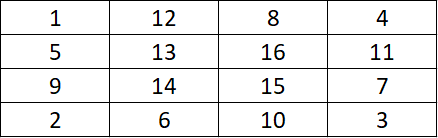
\includegraphics[height=50px]{n=4}
\end{center}

Apabila nilai $N = 5$, maka pola yang dihasilkan adalah seperti berikut
\begin{center}
    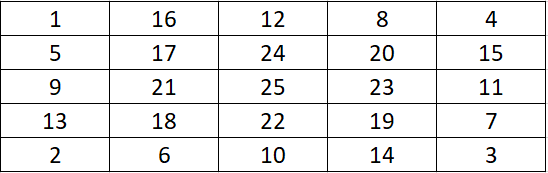
\includegraphics[height=50px]{n=5}
\end{center}

Lalu pertanyaan dari soal Elza adalah untuk pola dengan suatu suatu nilai $N$ tertentu, pada (baris,kolom) berapakah bilangan 
$K$ berada. Contoh apabila $N = 4$, maka bilangan $13$ ada pada sel (2, 2). 

Arvy lantas mengerjakan soal yang diberikan Elza tersebut dan setelah 1 jam akhirnya Arvy selesai menyelesaikannya.
Anda sebagai peserta babak final Arkavidia dapatkah menyelesaikan soal tersebut sama seperti Arvy?

\subsection*{Format Masukan}

Baris pertama terdiri dari satu bilangan bulat positif $T$ ($1 \leq T \leq 100.000$), menyatakan banyaknya kasus uji.
Tiap kasus uji terdiri dari dua bilangan bulat positif $N$ ($1 \leq N \leq 10^{9}$) dan $K$ ($1 \leq K \leq 10^{18}$)

\subsection*{Format Keluaran}

Untuk tiap kasus uji, keluarkan dua bilangan bulat positif $R$ dan $C$, yaitu posisi baris dan kolom bilangan $K$ berada pada 
pola untuk suatu nilai $N$.

\pagebreak

\begin{multicols}{2}
\subsection*{Contoh Masukan}
\begin{lstlisting}
3
4 1
4 6
4 15
\end{lstlisting}
\columnbreak
\subsection*{Contoh Keluaran}
\begin{lstlisting}
1 1
4 2
3 3
\end{lstlisting}
\vfill
\null
\end{multicols}

\subsection*{Penjelasan}
Pola yang dihasilkan adalah
\begin{center}
    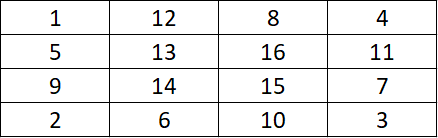
\includegraphics[height=50px]{n=4.PNG}
\end{center}
Sehingga bilangan 1 ada di (1,1), 6 ada di (4, 2), dan 15 ada di (3,3).

\pagebreak

\end{document}

